\usetikzlibrary{calc}

\begin{frame}{OSI model}
\begin{tikzpicture}
\node (osi) at (0,0) {
    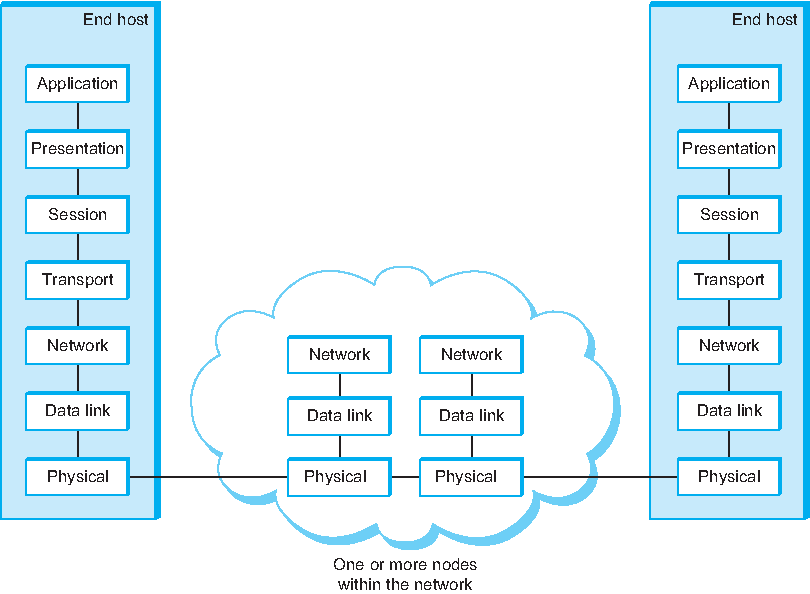
\includegraphics[height=0.75\textheight]{../intro/systemsapproach-1-fig-13.pdf}
};
\coordinate (explain loc) at ([xshift=0cm]osi.north east);
\tikzset{
    explain box/.style={alt=<2>{draw=red}{draw=black},very thick,align=left,at={(explain loc)}, anchor=north west},
    alt explain box={draw=red,anchor=north east,align=left=at{(explain loc)}
}
\begin{visibleenv}<2->
\node[explain box] {
    \myemph<3>{application}: \\ \hspace{.5cm}what requests/etc. \\
    \myemph<3>{presentation}: \\ \hspace{.5cm}format of data \\
    \myemph<3>{session}: \\ \hspace{.5cm}manage group of streams \\
    transport: \\ \hspace{.5cm}streams of data \\
    data link: \\ \hspace{.5cm}message $\rightarrow$ bits/\ldots \\
    physical: \\ \hspace{.5cm}send bits/\ldots 
};
\end{visibleenv}
\begin{visibleenv}<3>
\node[alt explain box] {
    current Internet \\
    usually these are all merged together \\
    (not actually seperate layers) \\
};
\end{visibleenv}
\begin{visibleenv}<3>
\node[alt explain box] {
};
\end{visibleenv}
\end{tikzpicture}
\imagecredit{Figure 13 of Chapter 1 of Computer Networks: A Systems Approach (6th ed) (Peterson and Davie)}
\end{frame}
